\documentclass{article}
\title{Web-based Supplementary Materials for Combinatorial Mixture Models for Single--Cell Assays with Application to Vaccine Studies by Greg Finak, SC De Rosa, Mario Roederer and Raphael Gottardo}

\usepackage{amssymb}
\usepackage{booktabs}
\usepackage{multirow,natbib}
\usepackage{url}
\def\bSig\mathbf{\Sigma}
\newcommand{\VS}{V\&S}
\newcommand{\tr}{\mbox{tr}}
\usepackage{amsmath,tikz}
\usetikzlibrary{calc}
\usetikzlibrary{positioning}
\date{}
\begin{document}
\maketitle
\appendix
%\renewcommand{\thesection}{\Alph{section}}
\renewcommand{\thesubsection}{Web Appendix \Alph{subsection}:}
%\setcounter{section}{1}
\setcounter{subsection}{0}
%\setcounter{figure}{0}
\renewcommand{\figurename}{\textbf{Web Figure}}
\renewcommand{\thefigure}{\textbf{\Alph{figure}}}
\setcounter{figure}{0}
%\todo[inline]{Note that the Supplementary Information section needs corrections to notation and overall}

\section*{}
\subsection{HVTN065 Vaccine Trial ICS Data Description}
\label{supp:statpublished}
HVTN065 is a phase 1 (safety and immunogenicity) trial of GeoVax HIV/AIDS DNA and MVA vaccine in 120 individuals (100 vaccinees, 20 placebo recipients, parts A and B). CD4 and CD8 T--cell epitope specific immune responses were measured via the ICS assay. Other humoral and cellular immune responses were measured via ELISA, and neutralizing antibody assays. Cytokines measured in the ICS assay included IFNg, TNFa, IL2, and IL4, and antigens included three Env, three Gag, and three Pol peptide pools. Results of the trial have been published~\citep{Goonetilleke:2006jk}.

%HVTN054 is a phase 1 (safety and immunogenicity) trial of an adenoviral vector vaccine in individuals without prior immunity~\cite{Peiperl:2010ej}. The vaccine vector expressed Gag, Pol and Env proteins from multiple HIV clades~\cite{Peiperl:2010ej}. Vaccine was given at two increasing doses, as well as a placebo. T--cell responses to antigens in the vaccine were measured via the ICS assay~\cite{Peiperl:2010ej,Horton:2007tsa}. The cytokines measured were IFNg (Interferon--$\gamma$), IL2 (Interleukin--2), TNFa (Tumor necrosis factor--$\alpha$) and IL4 (Interleukin 4)~\cite{Horton:2007tsa}. The sample size consisted of 20 vaccine and four placebo recipients. The original statistical analysis of the positivity calls is described in the associated publication~\cite{Peiperl:2010ej}. The Gag stimulated, IL2 expressing, CD4+ T--cell data from day 28 was used to derive hyper--parameter estimates for the simulation studies. 

\subsection{Constrained Beta--binomial model}
\label{supp:constrained}
We can define a model where we constrain the stimulated proportions under the alternative model such that $p_s>p_u$. In this case, the only changes required are for the alternative marginal likelihood $\mathrm{L}_1$ defined in equation~1. The marginal likelihood for the constrained model becomes $\mathrm{L}_1\times \mathrm{C}$, where $\mathrm{C}$ is a ratio of normalizing constants for the likelihood and the prior.

\begin{align*}
\begin{split}
	 \mathrm{C}=\frac{\int\limits_{p_{ui}=0}\limits^{1}\left(\frac{1}{\mathrm{B}(n_{ui}+\alpha_u,N_{ui}-n_{ui}+\beta_u)}p_{ui}^{n_{ui}+\alpha_u-1}(1-p_{ui})^{N_{ui}-n_{ui}+\beta_u-1} \right)\left(\mathrm{I_{1-p_{ui}}}(N^i_s-n^i_s+\beta_s,n^i_s+\alpha_s)\right)d p_{ui}}{   \int\limits_{p_{ui}=0}\limits^{1}\left(\frac{1}{\mathrm{B}(\alpha_u,\beta_u)}p_{ui}^{\alpha_u-1}(1-p_{ui})^{\beta_u-1} \right)\left(\mathrm{I_{1-p_{ui}}}(\beta_s,\alpha_s)\right)d p_{ui}}
%\label{eq:model2post}
\end{split}
\end{align*}
 
The term $I_{1-p_{ui}}(\beta_s,\alpha_s)=1-I_{p_{ui}}(\alpha_s,\beta_s)=Pr(p_{si} > p_{ui}; \alpha_s,\beta_s)$ is the regularized incomplete Beta function, which is just the CDF of a Beta distribution with parameters $\alpha_s,\beta_s$, resulting in a 1--dimensional integral that can be computed via Monte--Carlo integration (i.e. in our EM implementation). However, this can be computationally costly in the MCMC framework. In the latter case, we can compute the integral exactly if $\alpha_s$ and $\beta_s$ are integers by using the identity:
\begin{align}
I_{1-p_u}(\beta_s,\alpha_s) = \sum_{j=\beta_s}^{\beta_s+\alpha_s-1} \frac{(\beta_s+\alpha_s-1)!}{j!(\beta_s+\alpha_s-j)!}(1-p_u)^j(p_u)^{\beta_s+\alpha_s-j}
\label{eq:IBident}
\end{align}
Typically, in ICS data $\beta_s>>\alpha_s$, leading to relatively few terms in the sum in equation~\ref{eq:IBident}.  This leads to an exact expression for the normalizing constant:
$$
f
$$

\subsection{Derivation of Marginal Likelihoods for Beta--Binomial Model}

\subsection{The MCMC Algorithm}

\subsection{Marginal Likelihoods for the Multivariate Model}

\begin{figure} %  figure placement: here, top, bottom, or page
   \centering
%   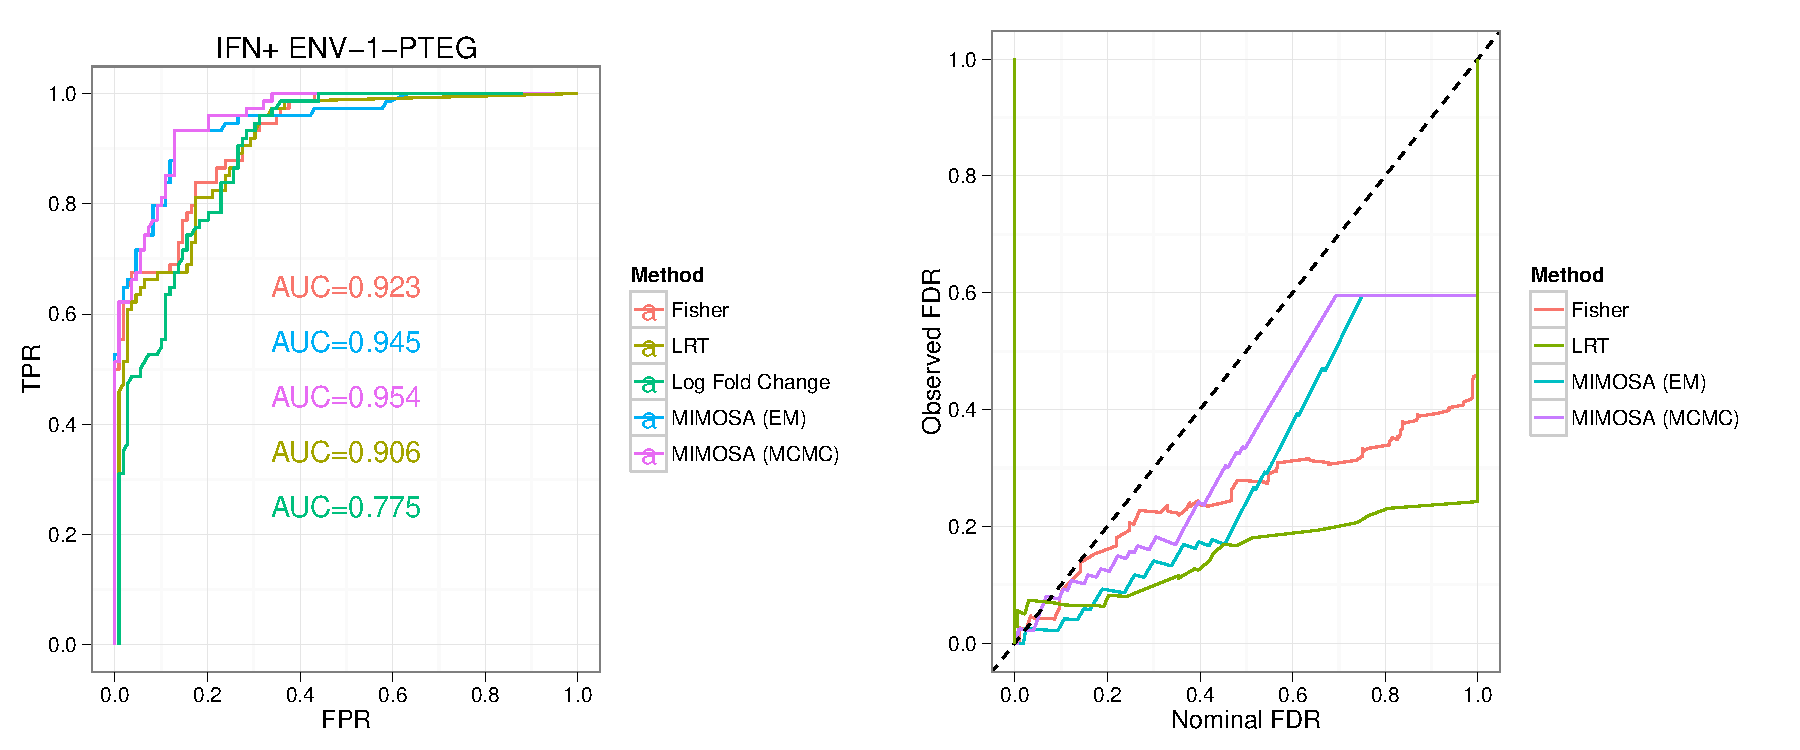
\includegraphics[width=.75\columnwidth]{Figures/2}\\ 
%   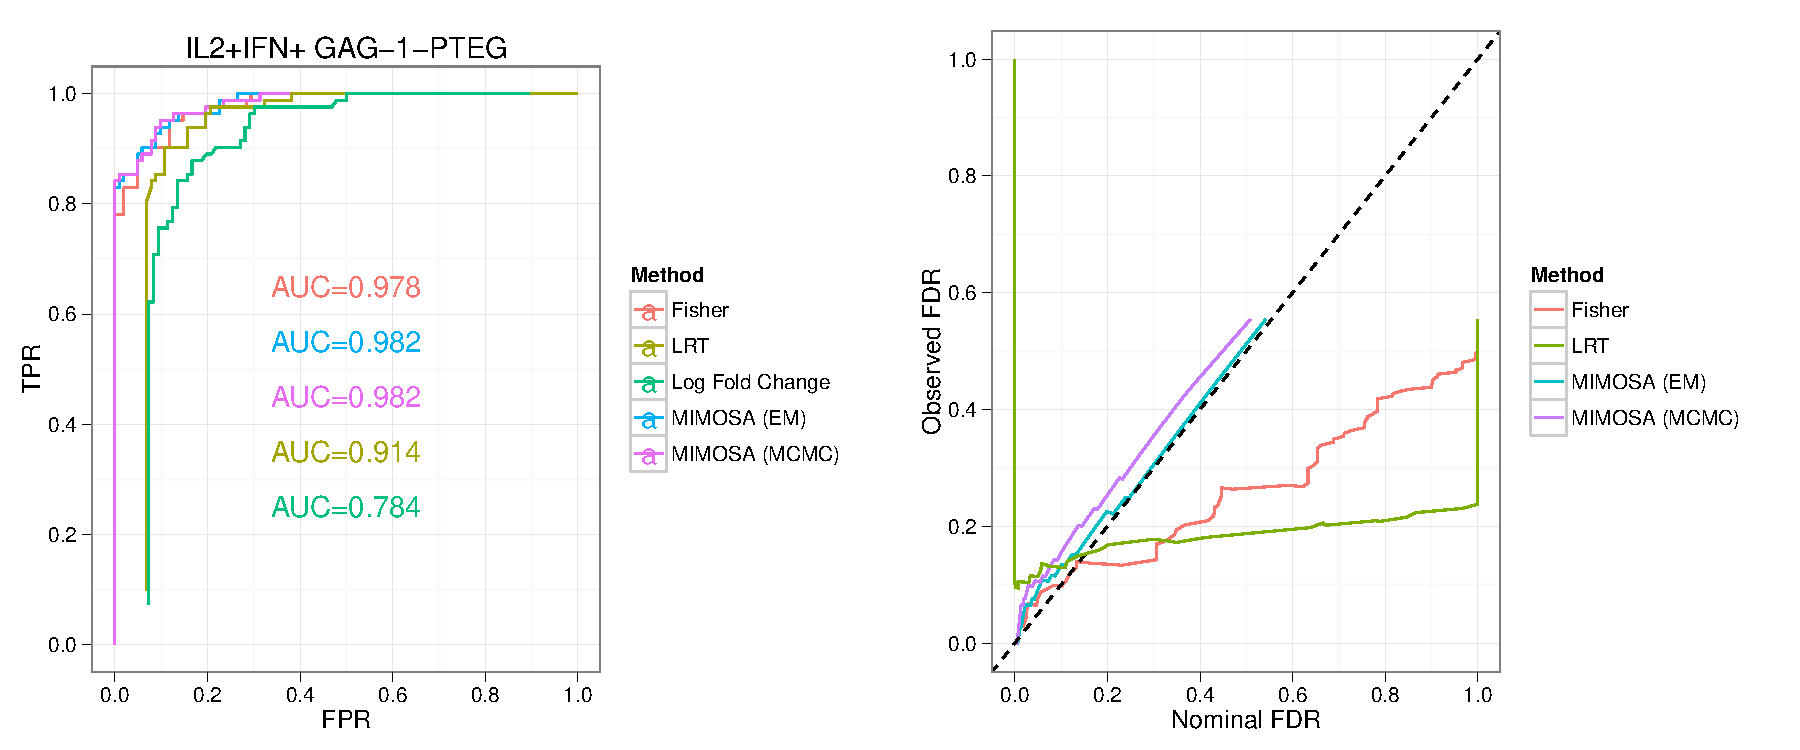
\includegraphics[width=.75\columnwidth]{Figures/12} 
\begin{tikzpicture} [auto, node distance=0cm]
\node at (0,0) (A){
\begin{tikzpicture}
    \node[anchor=south west,inner sep=0] at (0,0) (a) {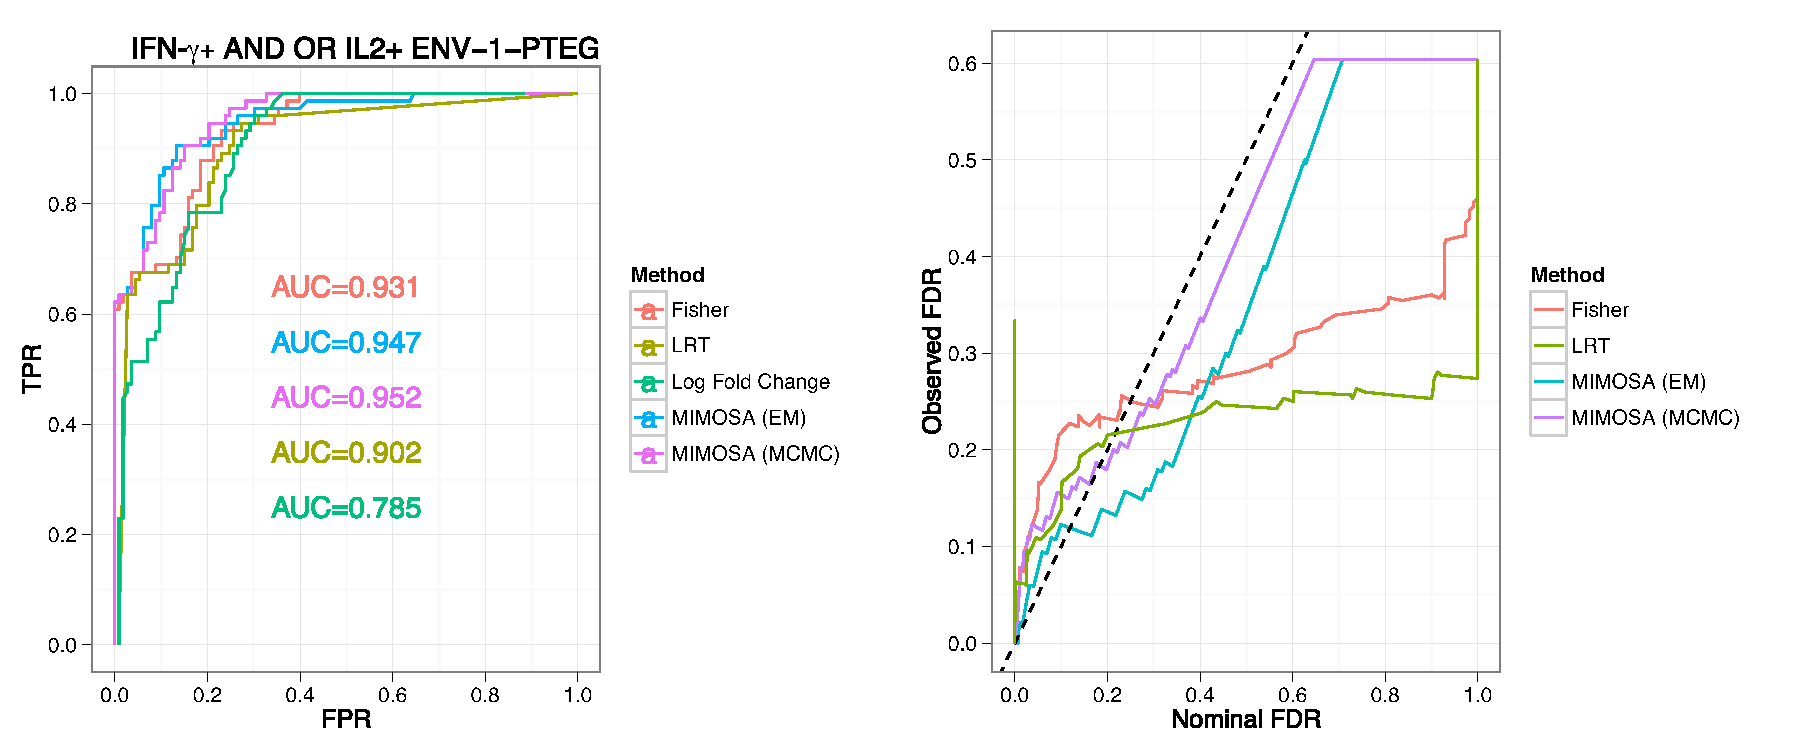
\includegraphics[width=.5\columnwidth]{Figures/15}};
    \begin{scope}[x={(a.south east)},y={(a.north west)}]
        \node at (0,1) [font=\tiny\sffamily] {A} ;
        \end{scope}
        \end{tikzpicture}
 };
 \node [right=of A] (B) {
 \begin{tikzpicture}
    \node[anchor=south west, inner sep=0] at (0,0) (b) {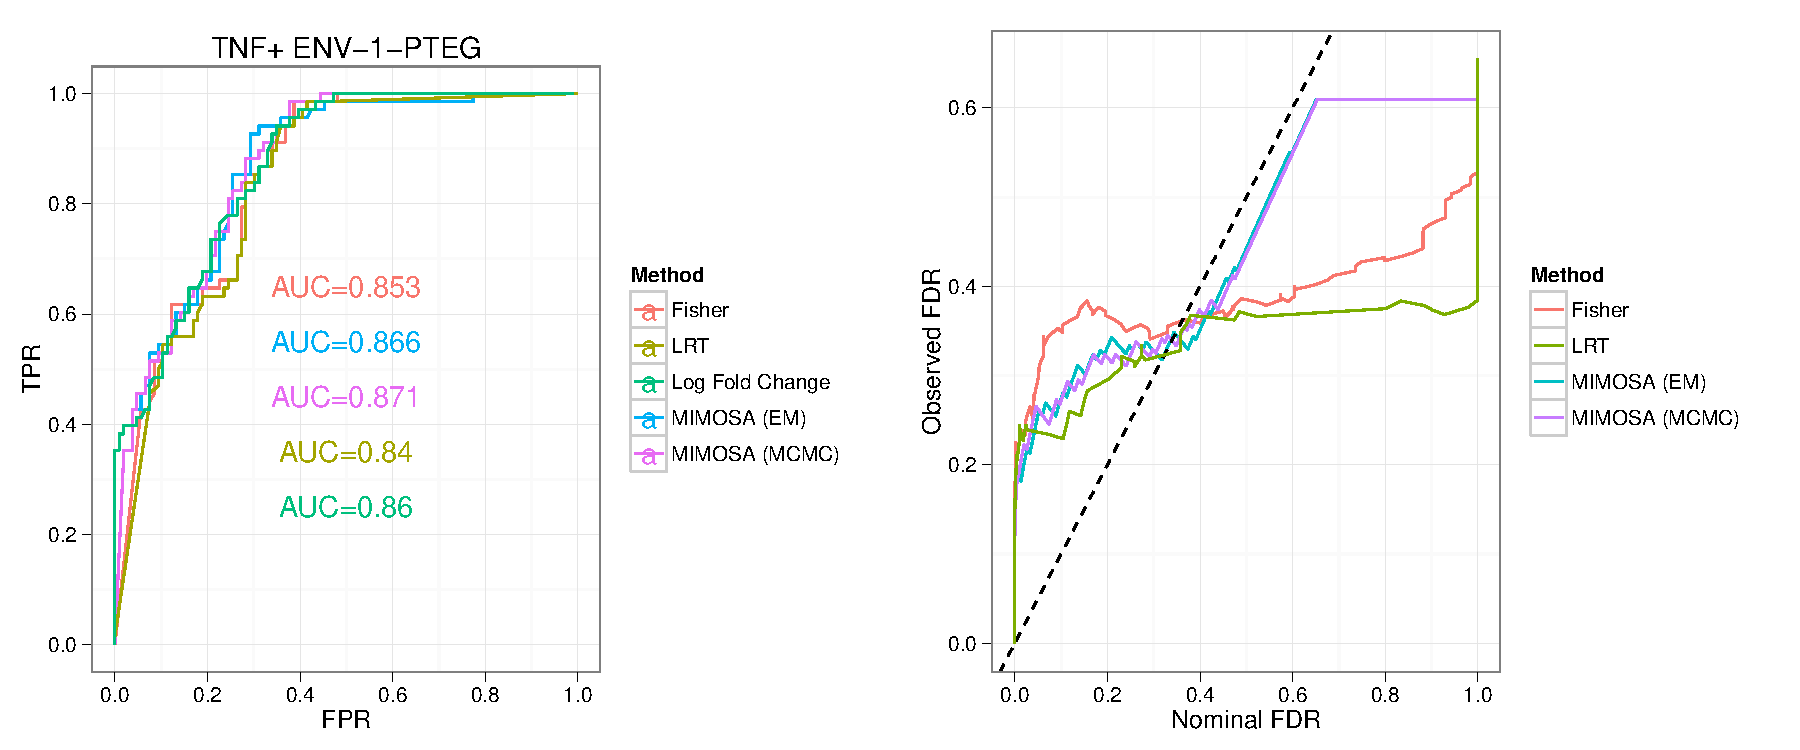
\includegraphics[width=.5\columnwidth]{Figures/3}};
        \begin{scope}[x={(b.south east)},y={(b.north west)}]
        \node at (0,1) [font=\tiny\sffamily] {B} ;
                \end{scope}
        \end{tikzpicture}
 };
 \node [below=of A] (C) {
 \begin{tikzpicture}
    \node[anchor=south west, inner sep=0] at (0,0) (c) {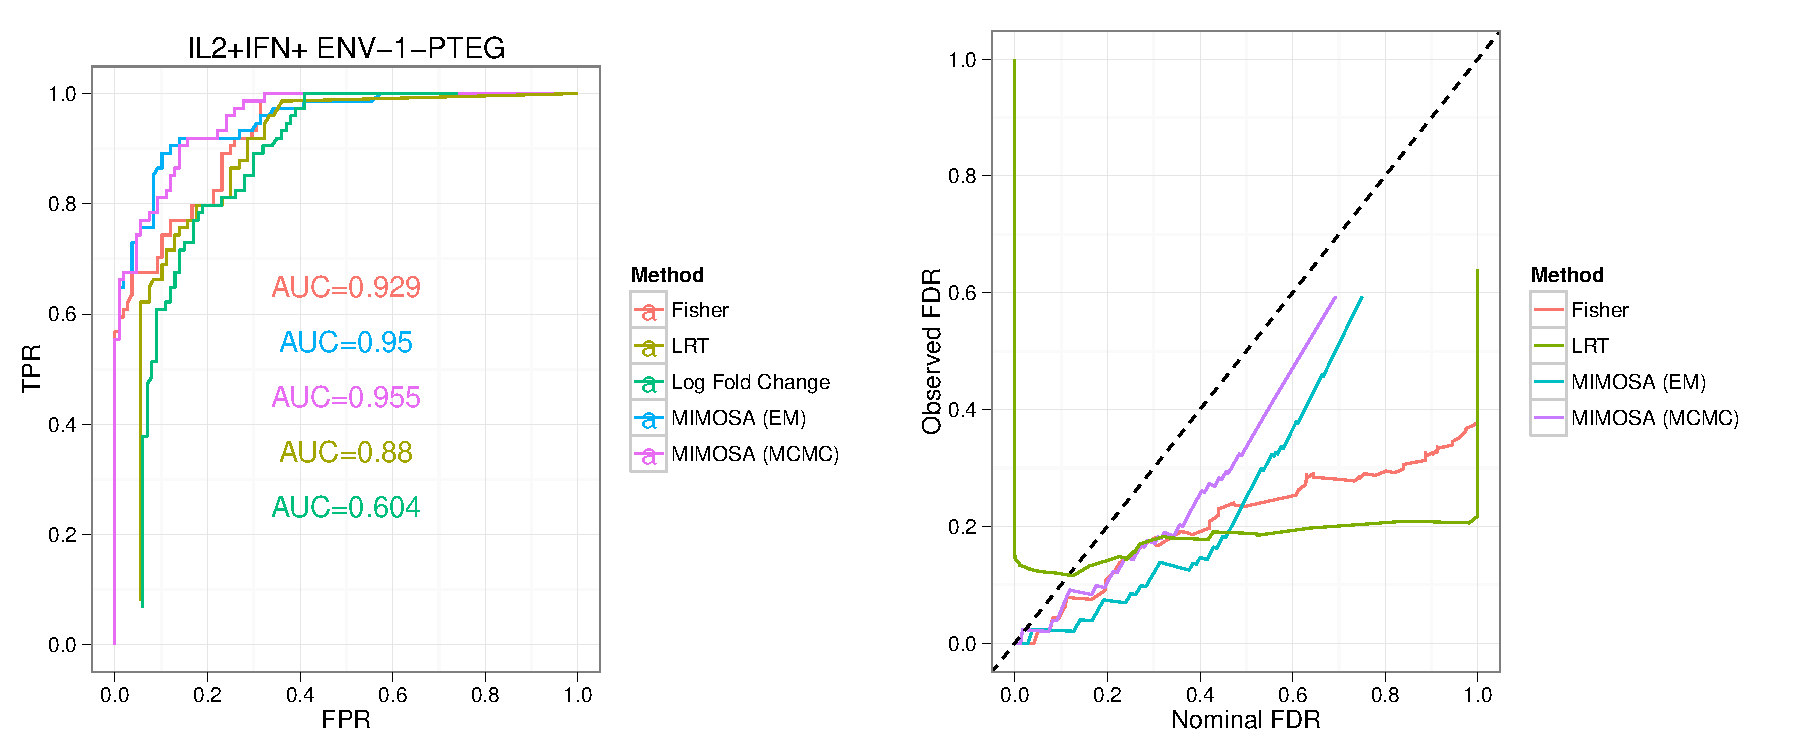
\includegraphics[width=.5\columnwidth]{Figures/5}};
        \begin{scope}[x={(c.south east)},y={(c.north west)}]
        \node at (0,1) [font=\tiny\sffamily] {C} ;
        \end{scope}
        \end{tikzpicture}
};
\node [below=of B] (D) {
\begin{tikzpicture}
    \node[anchor=south west, inner sep=0] at (0,0) (d) {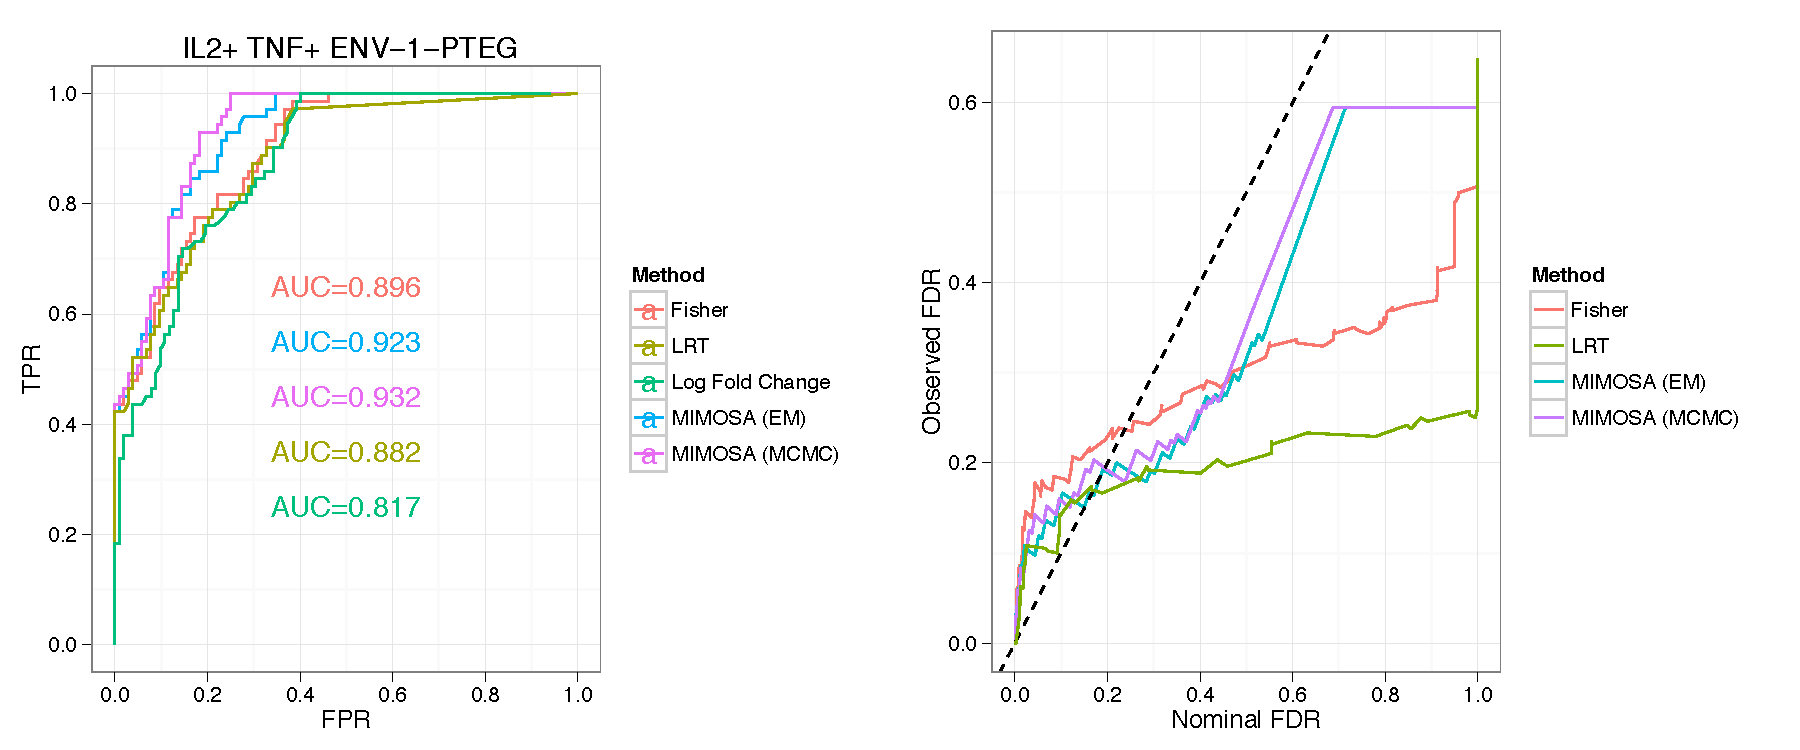
\includegraphics[width=.5\columnwidth]{Figures/6}};
        \begin{scope}[x={(d.south east)},y={(d.north west)}]
        \node at (0,1) [font=\tiny\sffamily] {D} ;
                \end{scope}
        \end{tikzpicture}
};
\node [below=of C] (E) {
\begin{tikzpicture}
    \node[anchor=south west, inner sep=0] at (0,0) (e) {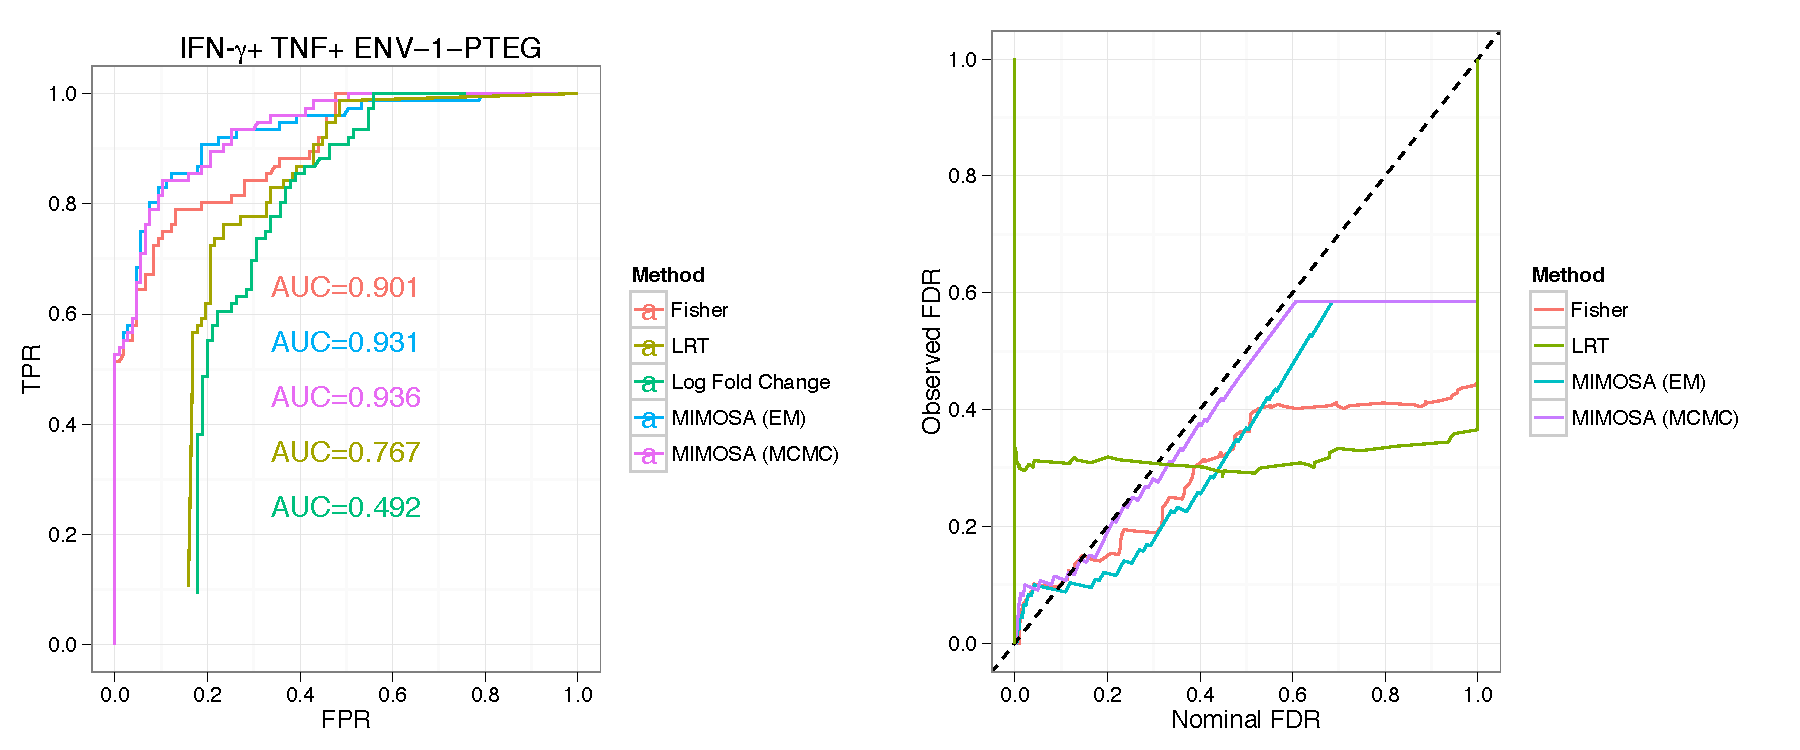
\includegraphics[width=.5\columnwidth]{Figures/7}};
        \begin{scope}[x={(d.south east)},y={(d.north west)}]
        \node at (0,1) [font=\tiny\sffamily] {E} ;
                \end{scope}
        \end{tikzpicture}
 };
   % \node[anchor=south west, inner sep=0] at (8,-7.5){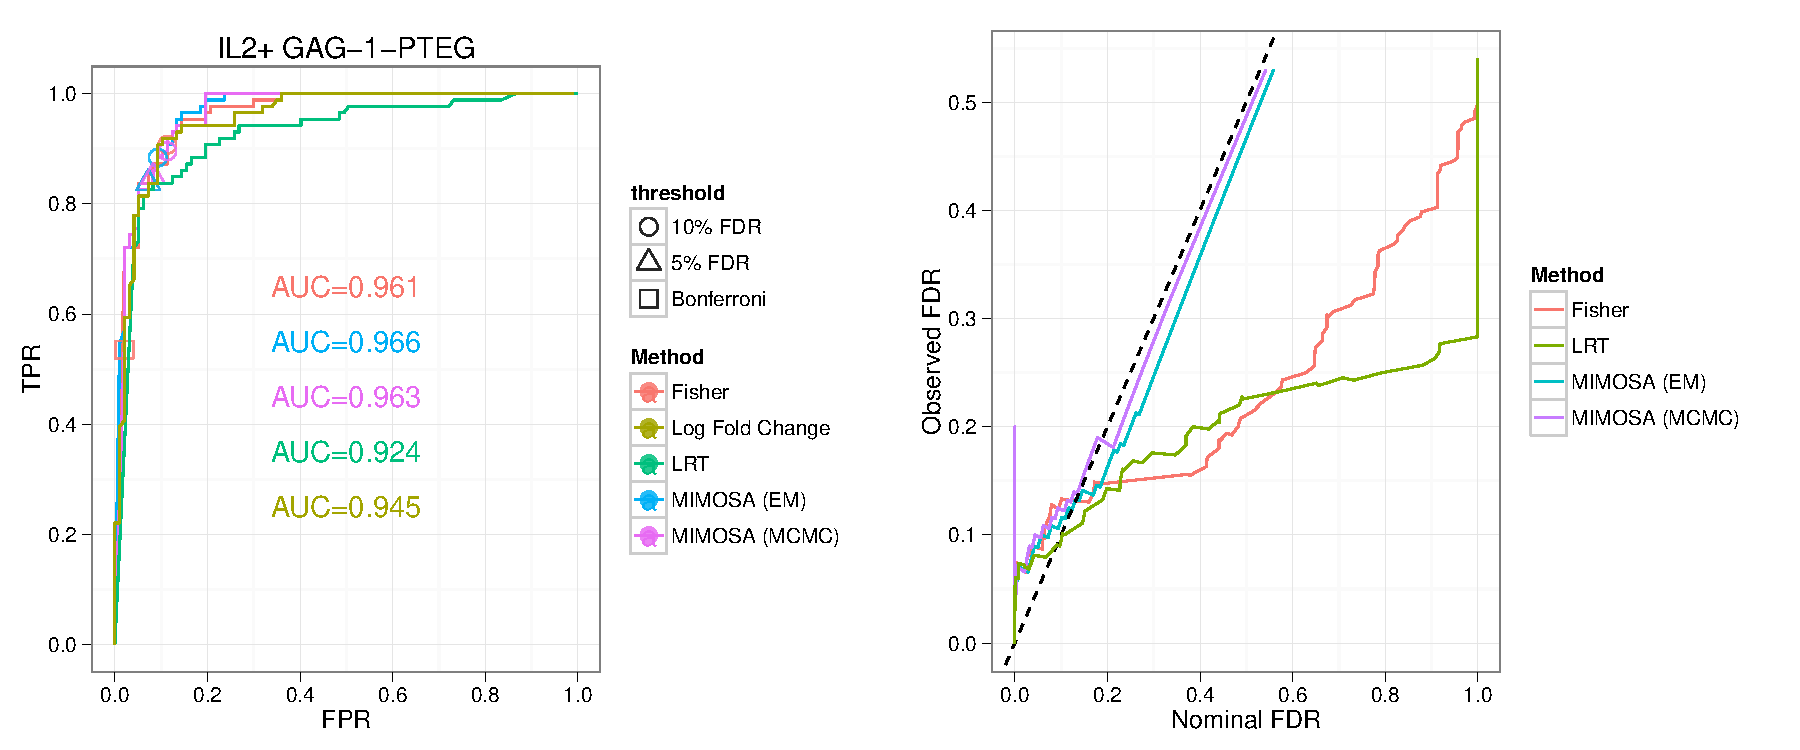
\includegraphics[width=.5\columnwidth]{Figures/8}};
   % \node[anchor=south west, inner sep=0] at (0,-11.25){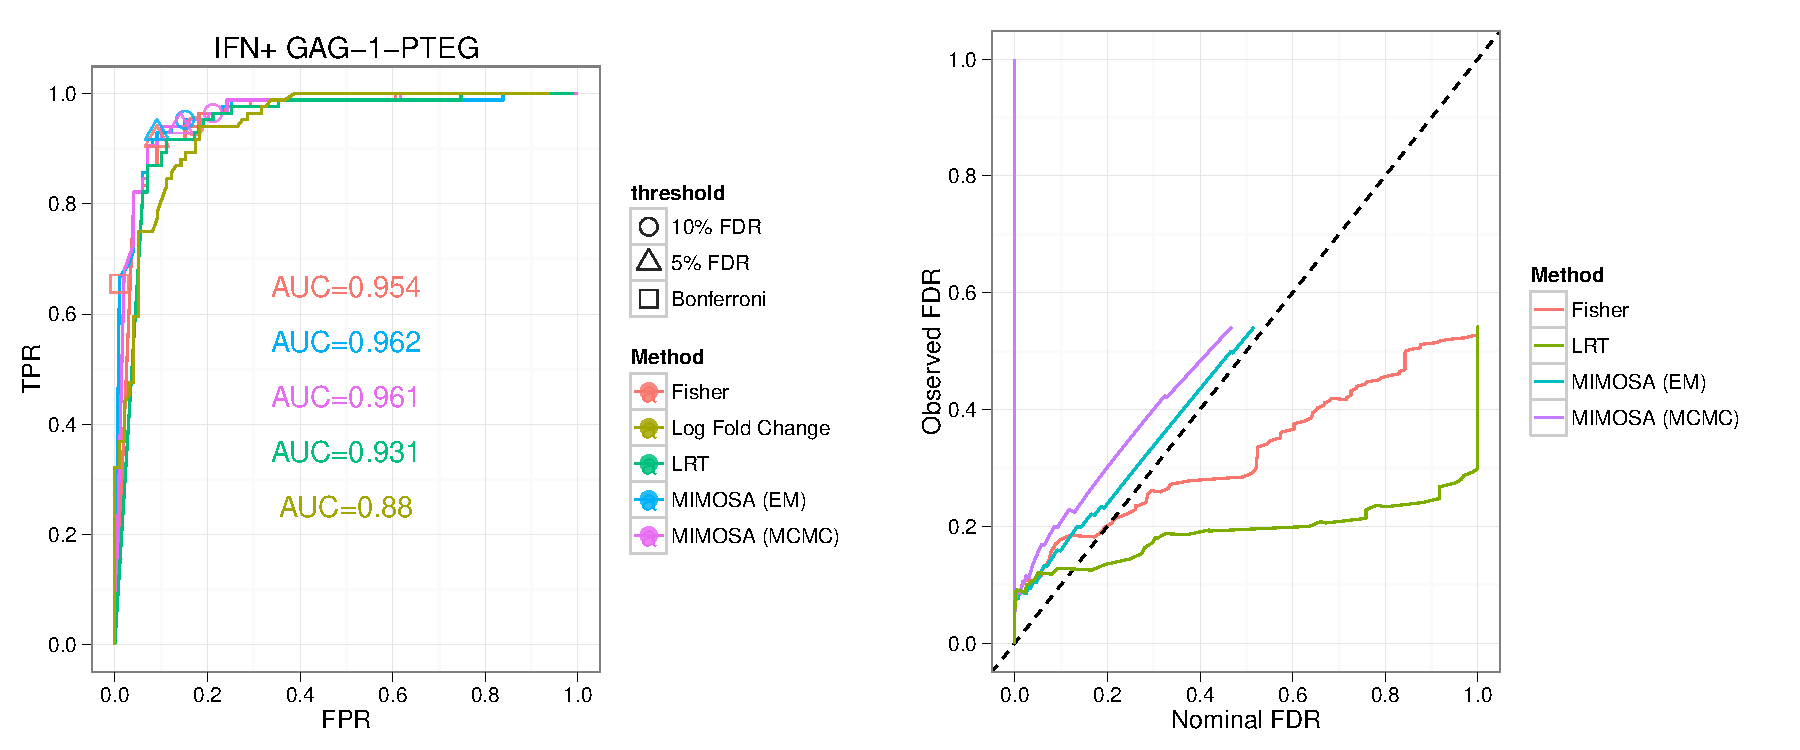
\includegraphics[width=.5\columnwidth]{Figures/9}};
    %\node[anchor=south west, inner sep=0] at (8,-11.25){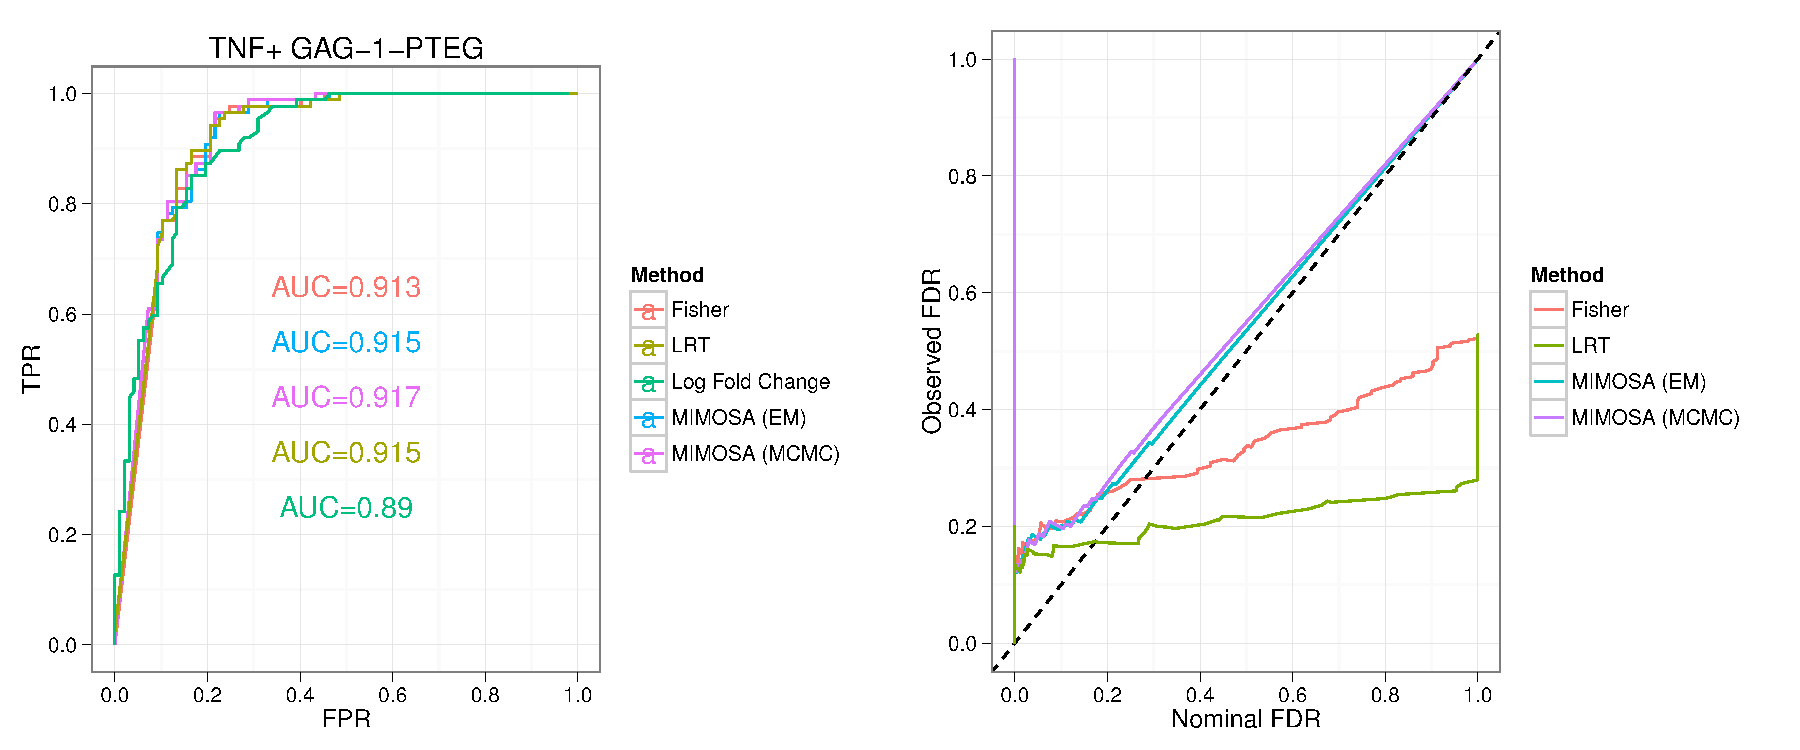
\includegraphics[width=.5\columnwidth]{Figures/10}};
    %\node[anchor=south west, inner sep=0] at (0,-15){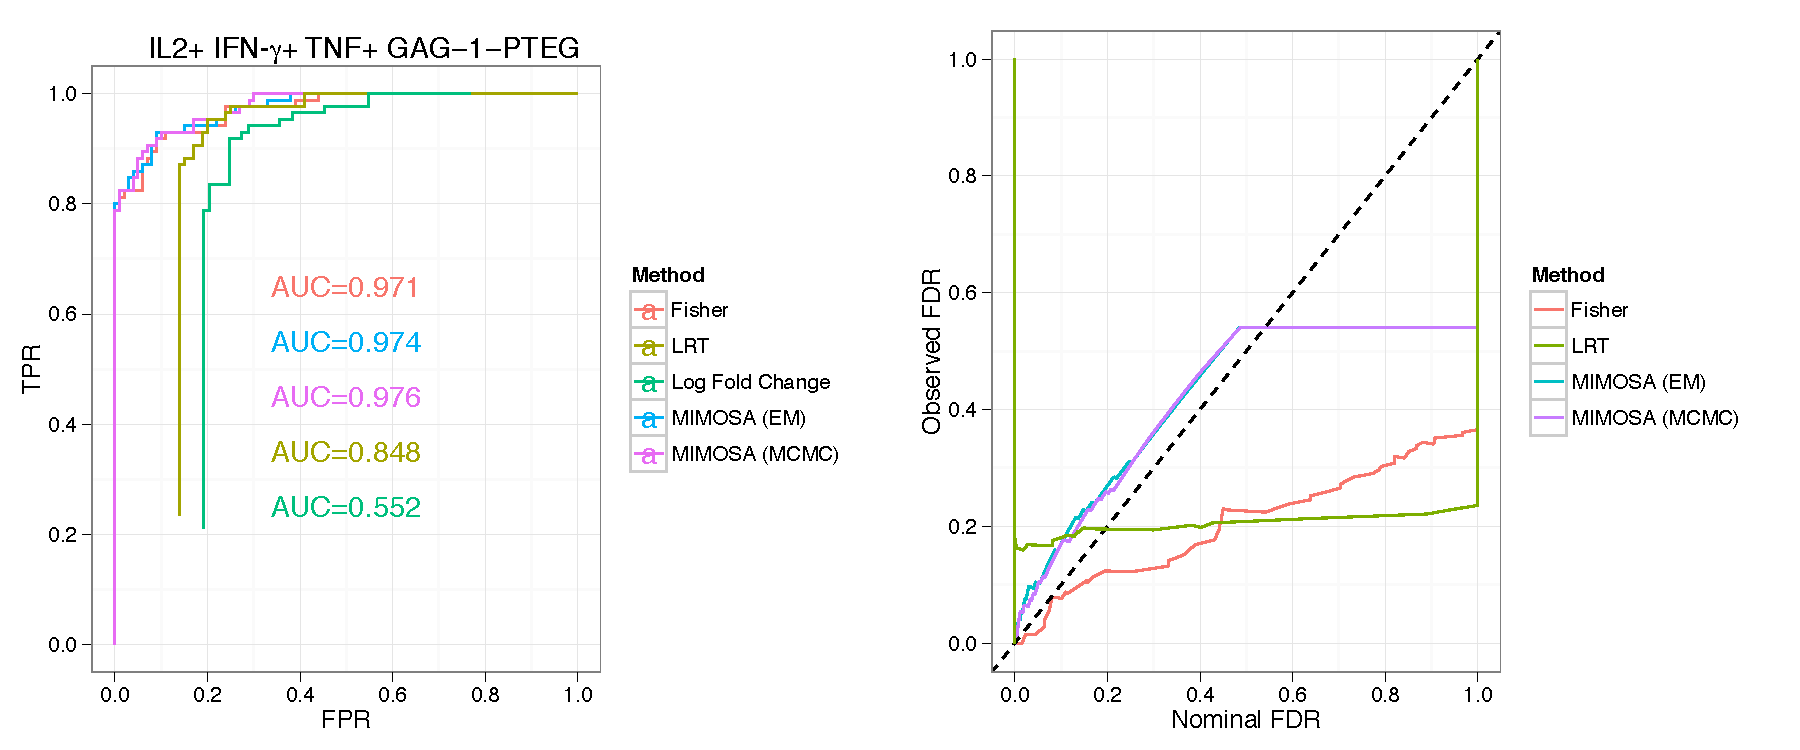
\includegraphics[width=.5\columnwidth]{Figures/11}};
    %\node[anchor=south west, inner sep=0] at (8,-15){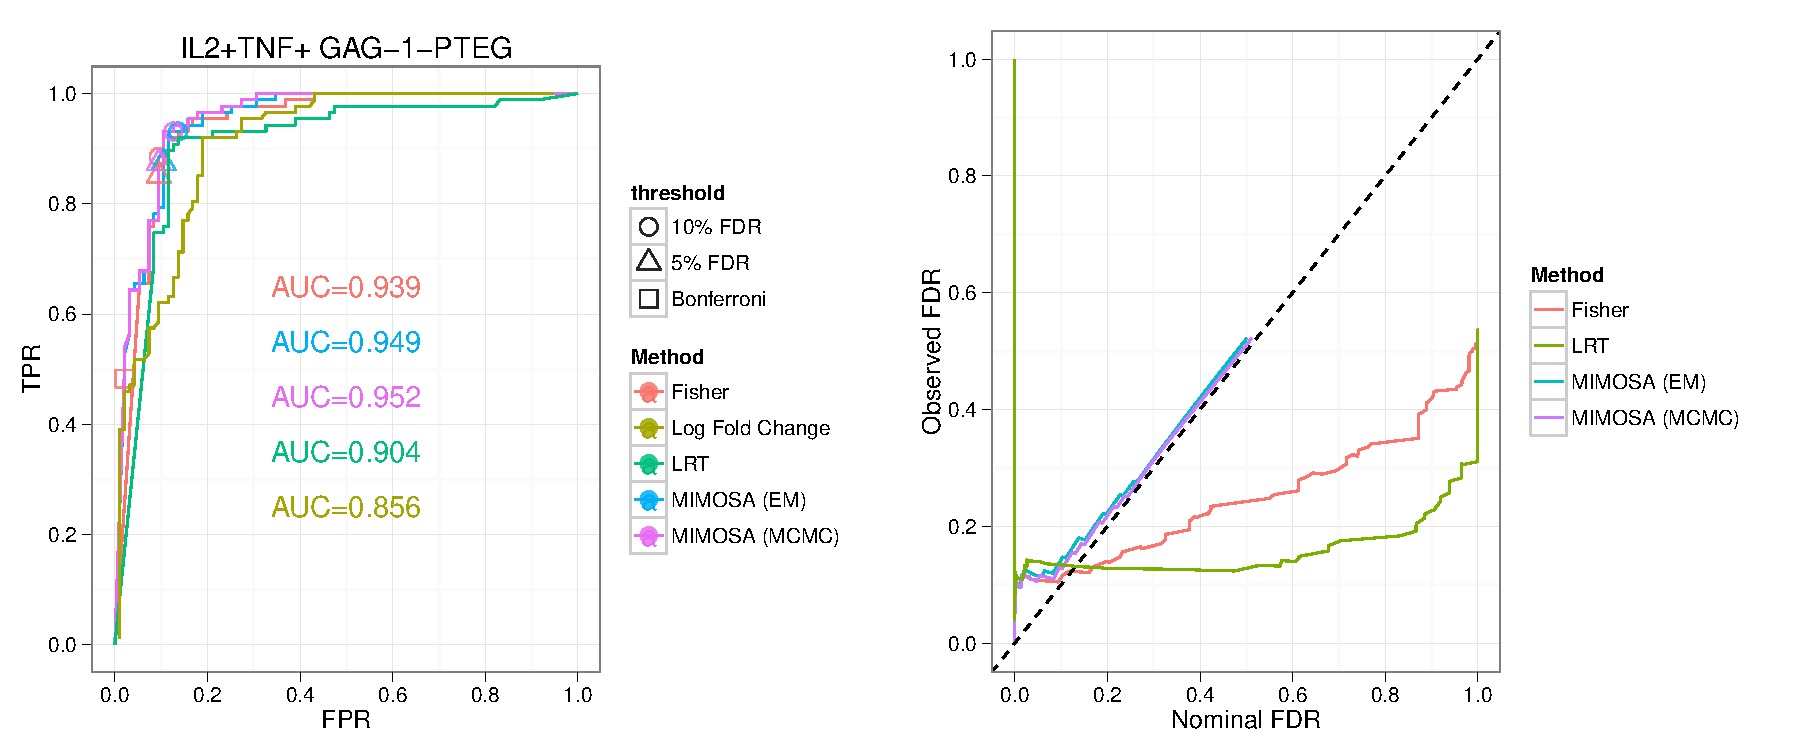
\includegraphics[width=.5\columnwidth]{Figures/13}};

  %  \node at (8,-4) [font=\tiny\sffamily] {F} ;
%    \node at (0,-7.75) [font=\tiny\sffamily] {G} ;
  %  \node at (8,-7.75) [font=\tiny\sffamily] {H} ;
   % \node at (0,-11.75) [font=\tiny\sffamily] {I} ;
   % \node at (8,-11.75) [font=\tiny\sffamily] {J} ;
    \end{tikzpicture}
   \caption{Comparison of MIMOSA on other cytokines and cytokine combinations for ENV-1-PTEG stimulated CD4+ T-cells from the HVTN065 trial.}
\label{webfig:HVTN065Results}
\end{figure}

%\begin{figure}[htbp] %  figure placement: here, top, bottom, or page
%   \centering
%%   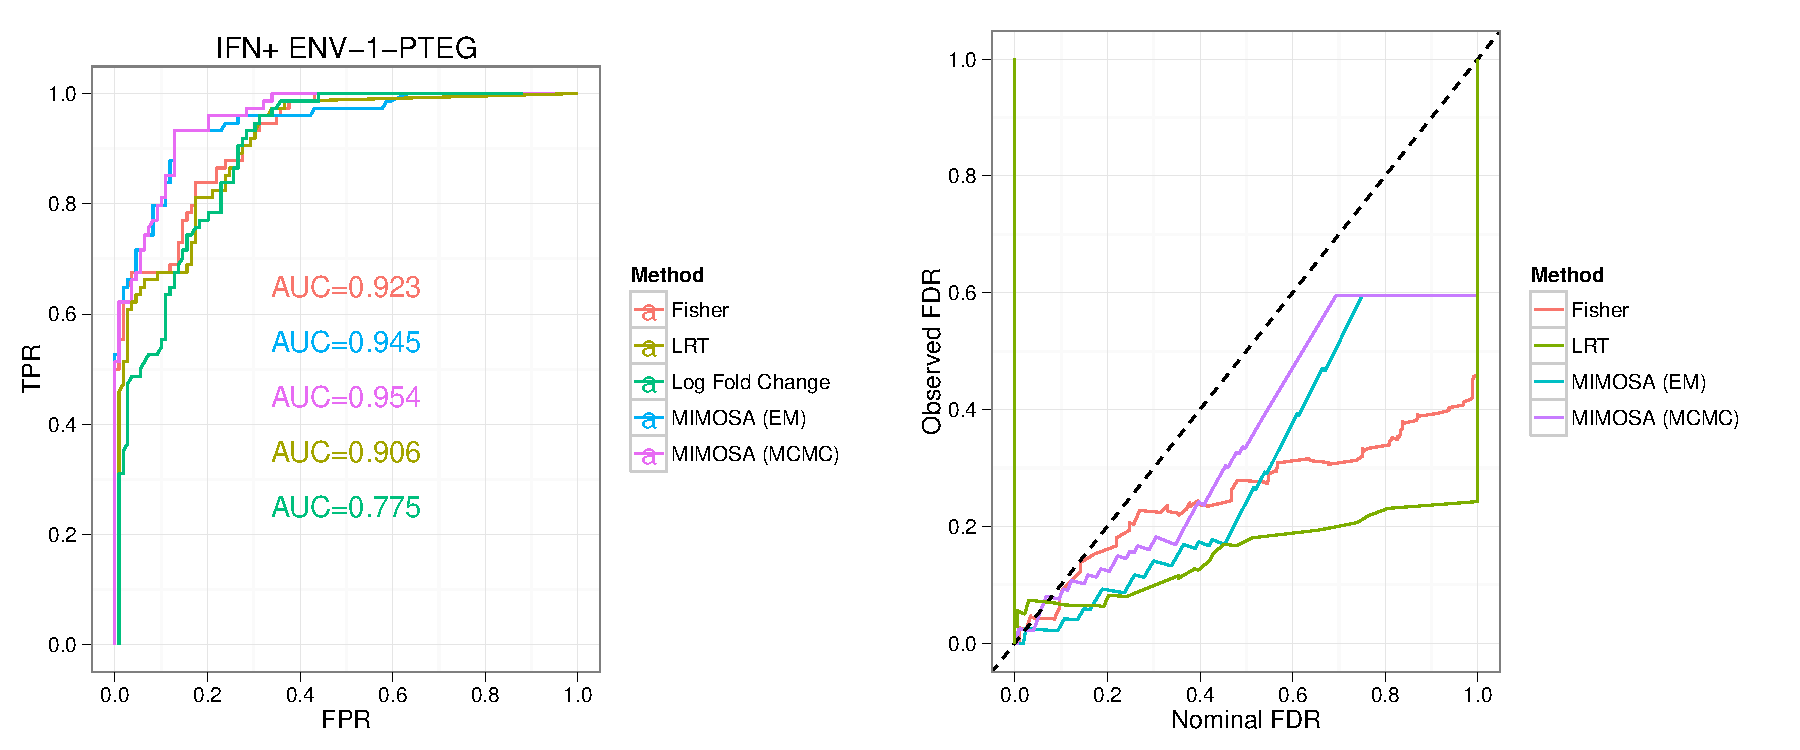
\includegraphics[width=.75\columnwidth]{Figures/2}\\ 
%%   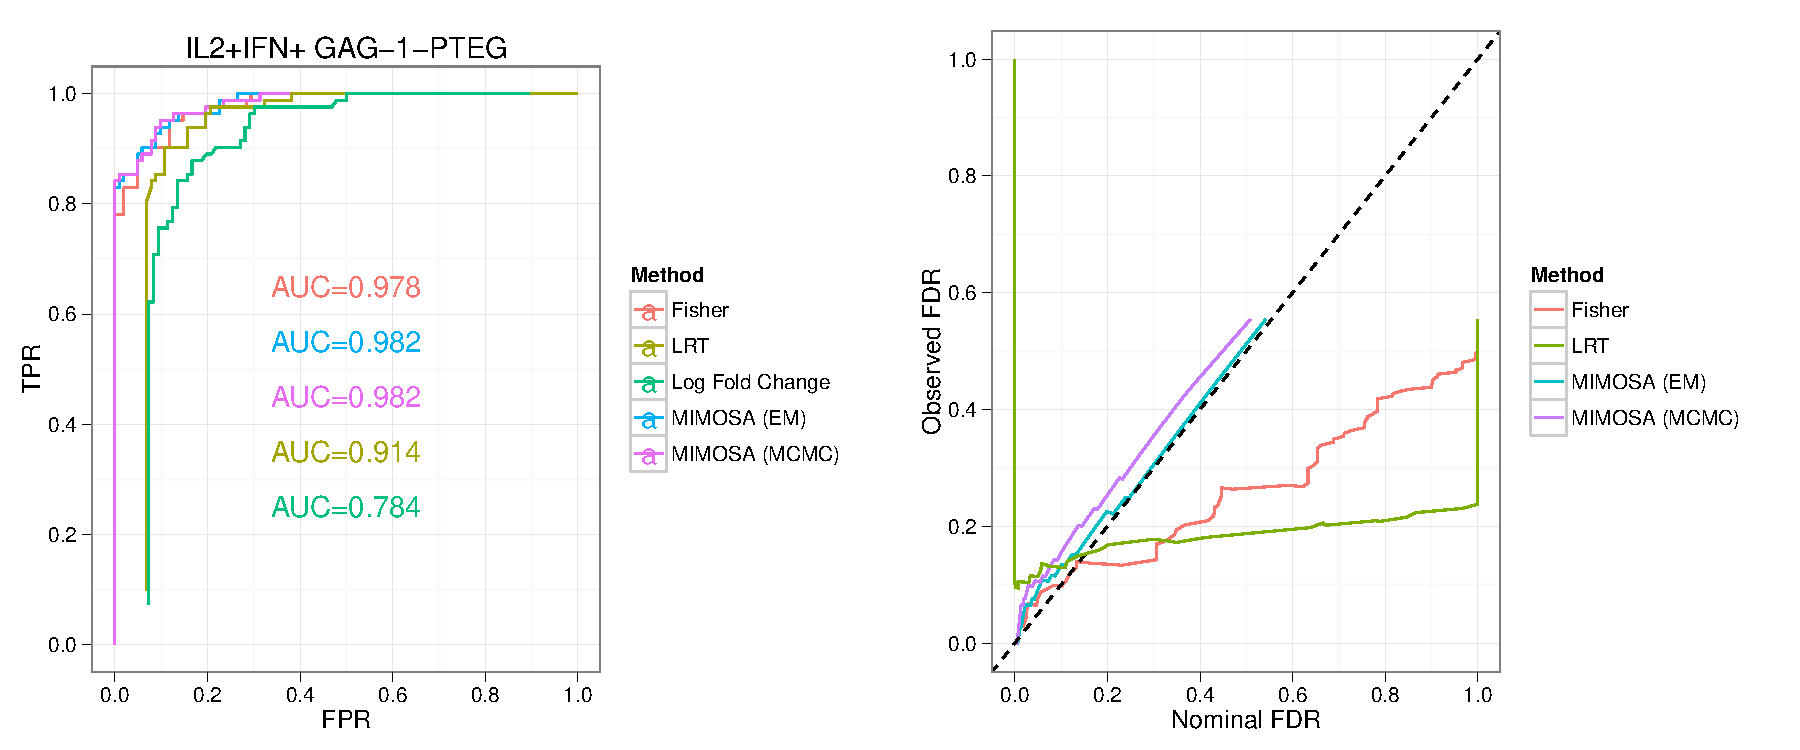
\includegraphics[width=.75\columnwidth]{Figures/12} 
%\begin{tikzpicture}
%    \node[anchor=south west, inner sep=0] at (0,0){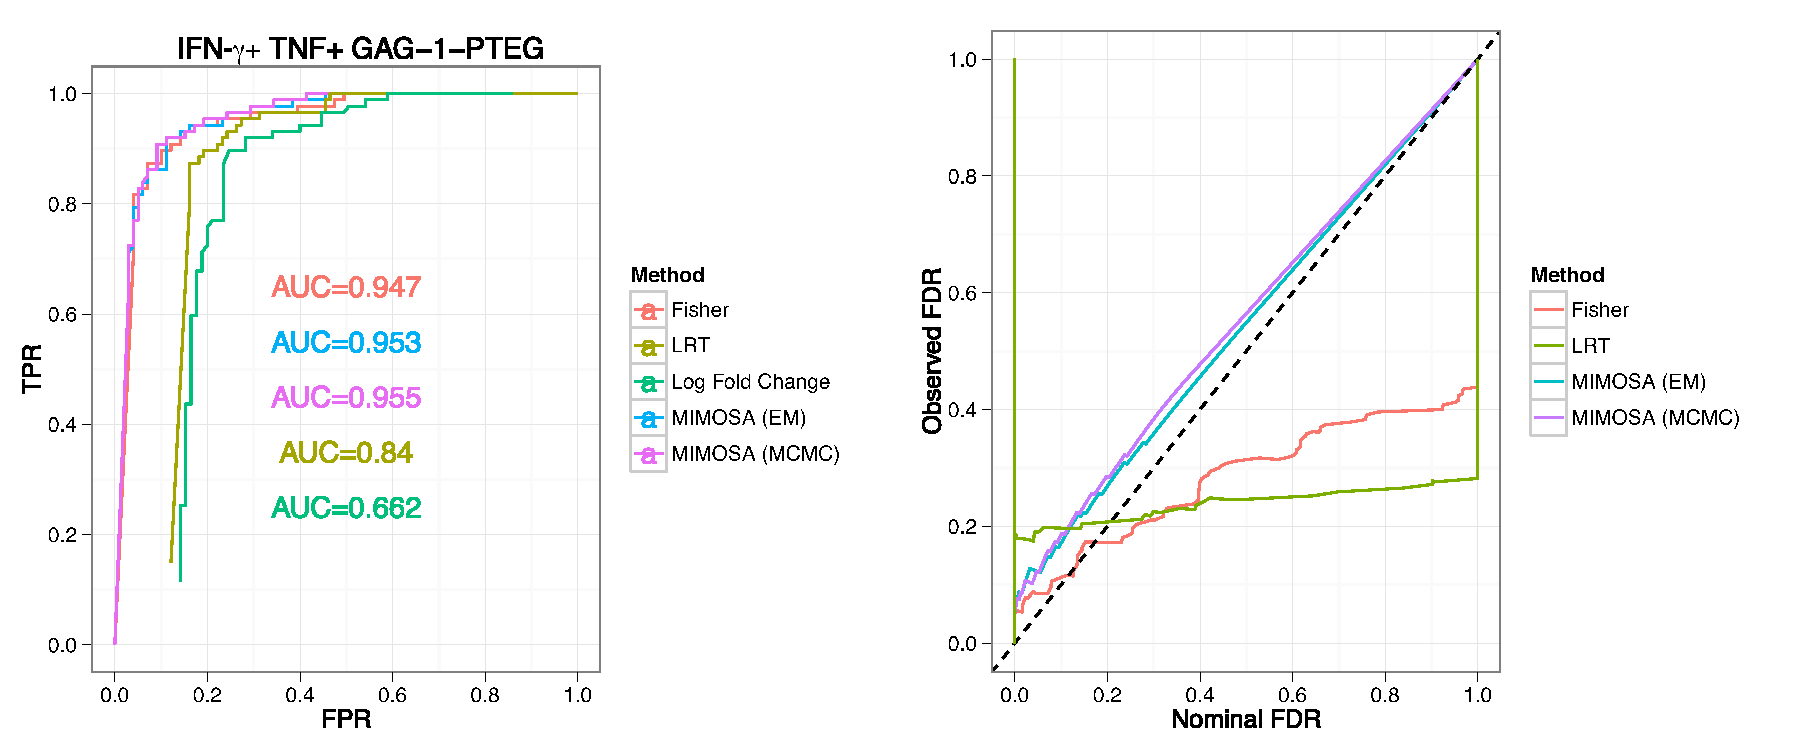
\includegraphics[width=.5\columnwidth]{Figures/14}};
%    \node[anchor=south west, inner sep=0] at (8,0){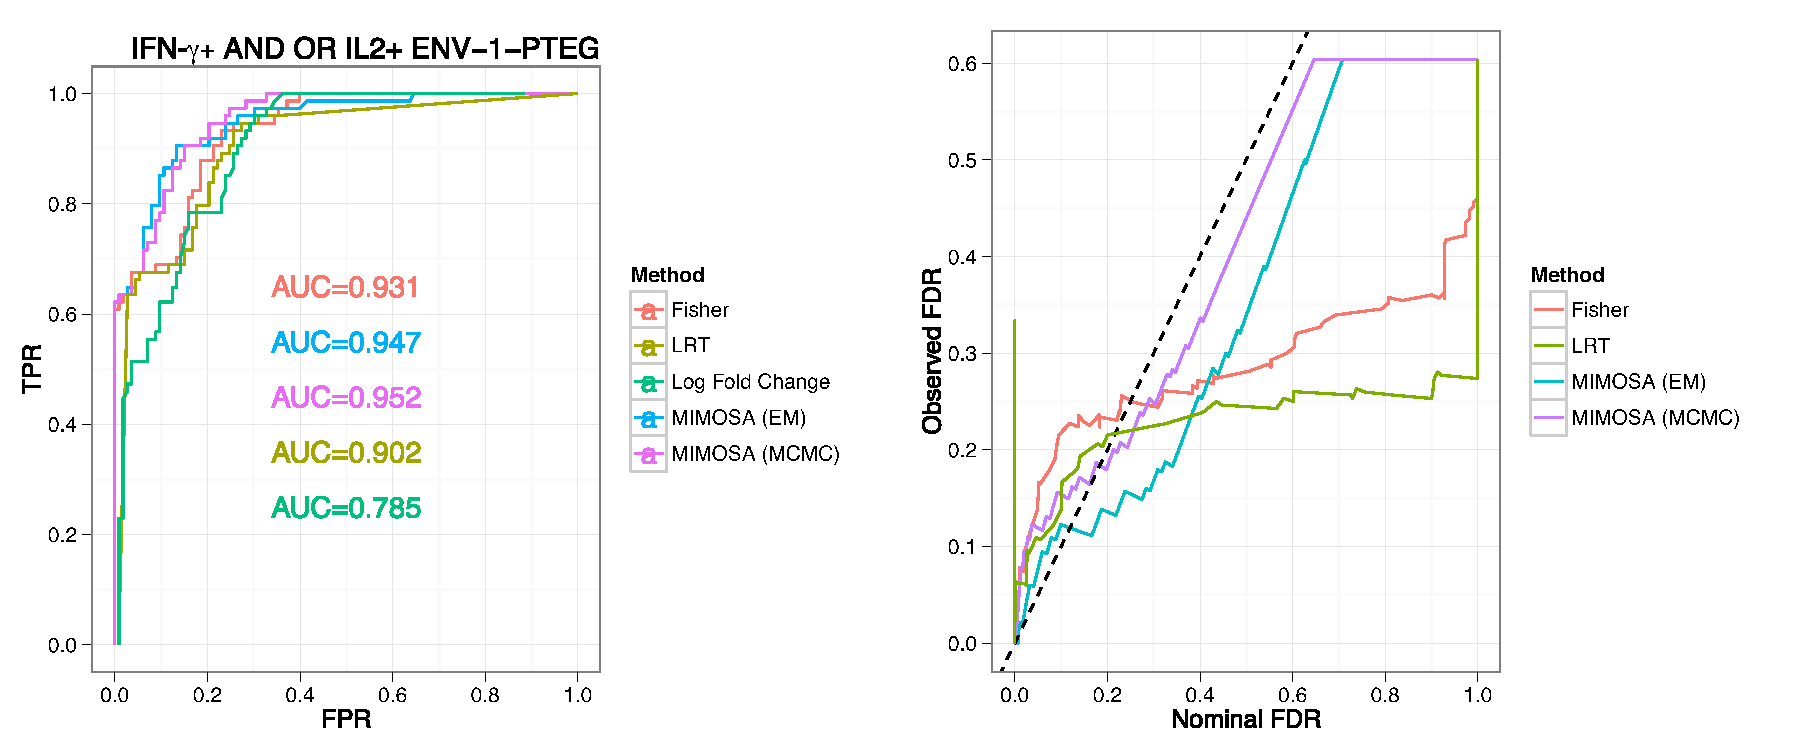
\includegraphics[width=.5\columnwidth]{Figures/15}};
%    \node[anchor=south west, inner sep=0] at (0,-3.75){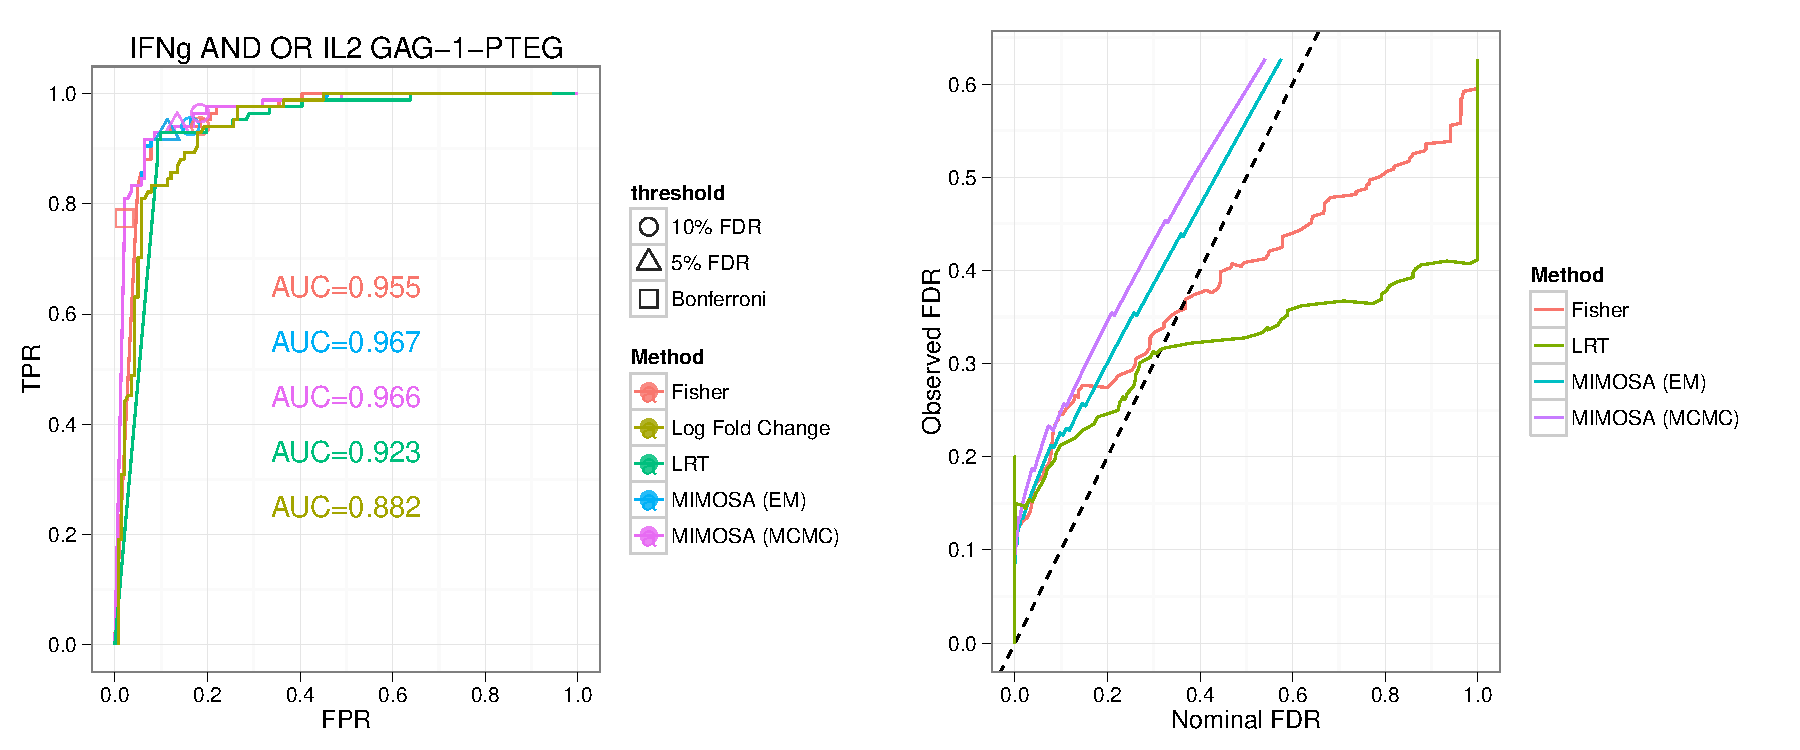
\includegraphics[width=.5\columnwidth]{Figures/16}};
%
%
%    \node at (0,3.4) [font=\tiny\sffamily] {A} ;
%    \node at (8,3.4) [font=\tiny\sffamily] {B} ;
%    \node at (0,-0.5) [font=\tiny\sffamily] {C} ;
%    \end{tikzpicture}
%   \caption{Comparison of MIMOSA on other cytokines and cytokine combinations for ENV-1-PTEG and GAG-1-PTEG stimulated CD4+ T-cells from the HVTN065 trial.}
%\label{fig:HVTN065ResultsCont}
%\end{figure}

\begin{figure} %  figure placement: here, top, bottom, or page
   \centering
\begin{tikzpicture} [auto,node distance=0cm]
\node at (0,0) (A) {
\begin{tikzpicture}
    \node[anchor=south west,inner sep=0] at (0,0) (a) {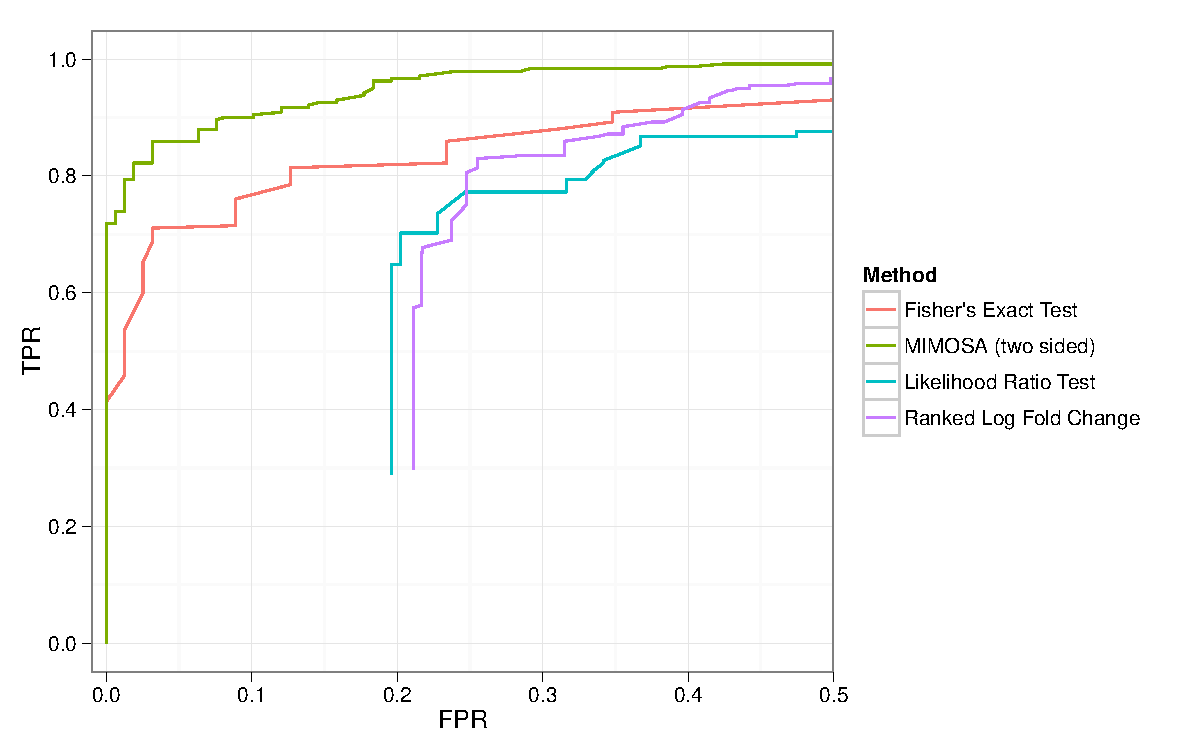
\includegraphics[width=0.4\columnwidth]{Figures/Sim_Twosided_ROC_5000.pdf}};
    \begin{scope} [x={(a.south east)},y={(a.north west)}]
        \node at (0,1) [font=\tiny\sffamily] {A} ;
    \end{scope}
    \end{tikzpicture}
    };
    \node [right=of A] (B) {
    \begin{tikzpicture}
    \node[anchor=south west, inner sep=0] at (0,0) (b) {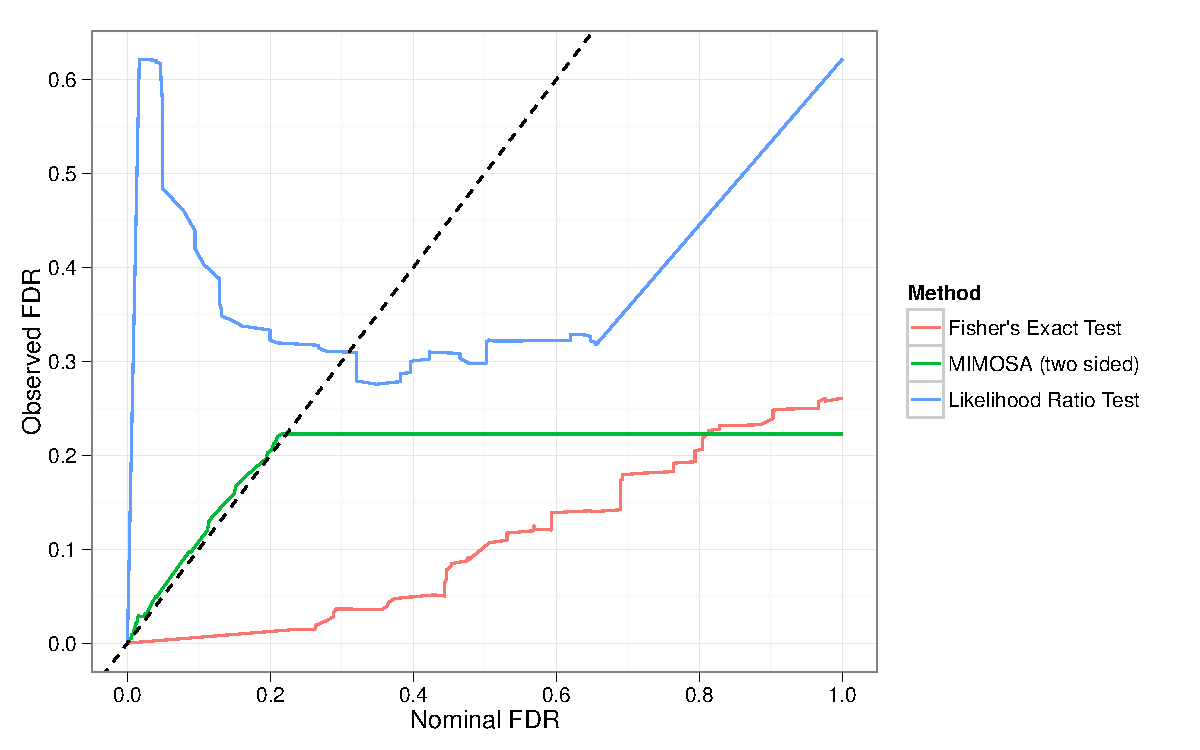
\includegraphics[width=0.4\columnwidth]{Figures/Sim_Twosided_FDR_5000.pdf}};
        \begin{scope} [x={(b.south east)},y={(b.north west)}]
        \node at (0,1) [font=\tiny\sffamily] {B} ;
        \end{scope}
    \end{tikzpicture}
    };
    \node [below=of A] (C) {
    \begin{tikzpicture}
     \node[anchor=south west,inner sep=0] at (0,0) (c) {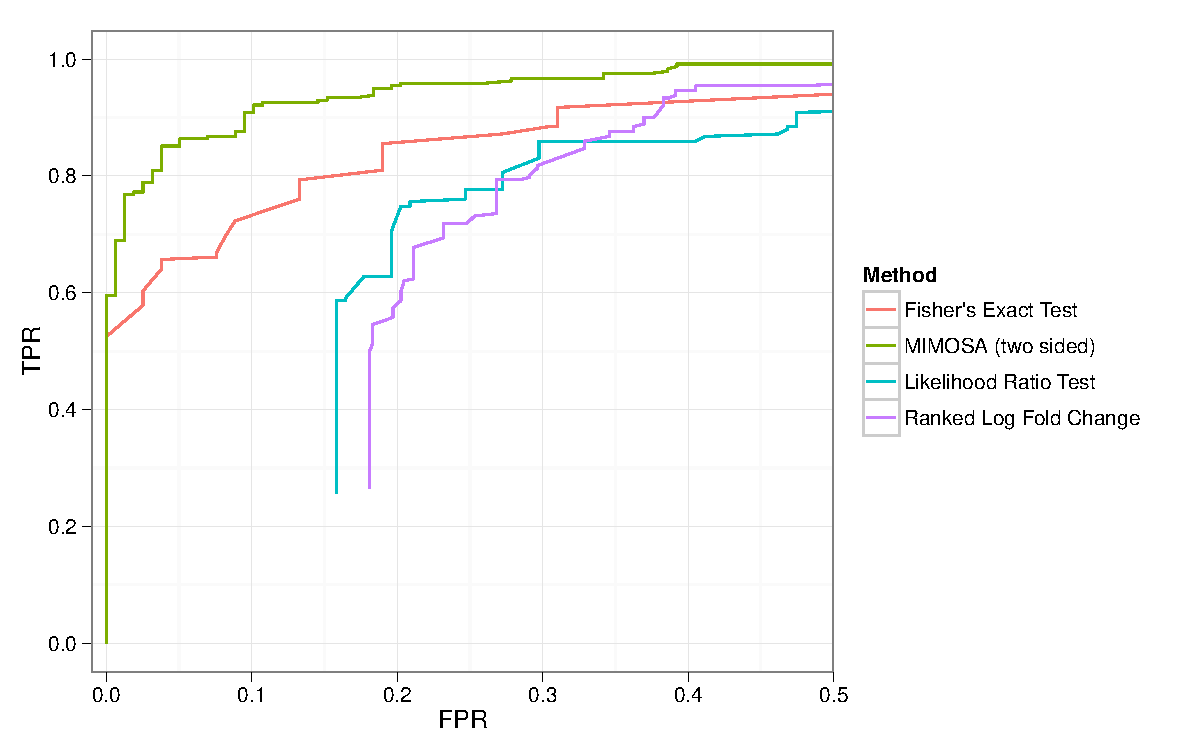
\includegraphics[width=0.4\columnwidth]{Figures/Sim_Truncated_ROC_5000.pdf}};
         \begin{scope} [x={(c.south east)},y={(c.north west)}]
                 \node at (0,1) [font=\tiny\sffamily] {C} ;
	\end{scope}
     \end{tikzpicture}
     };
     \node [below=of B] (D) {
     \begin{tikzpicture}
    \node[anchor=south west, inner sep=0] at (0,0) (d) {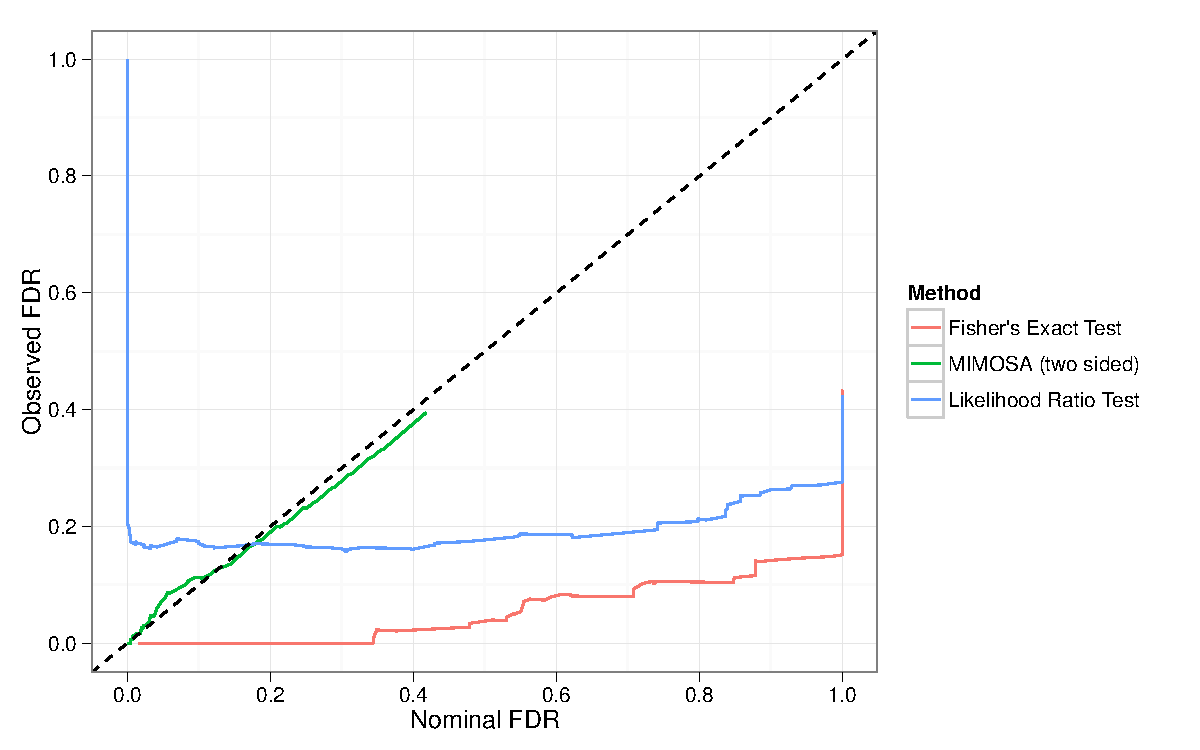
\includegraphics[width=0.4\columnwidth]{Figures/Sim_Truncated_FDR_5000.pdf}};
        \begin{scope} [x={(d.south east)},y={(d.north west)}]
            \node at (0,1) [font=\tiny\sffamily] {D} ;
\end{scope}
    \end{tikzpicture}
    };
  \node [below=of C] (E) {
\begin{tikzpicture}
    \node[anchor=south west,inner sep=0] at (0,0) (e) {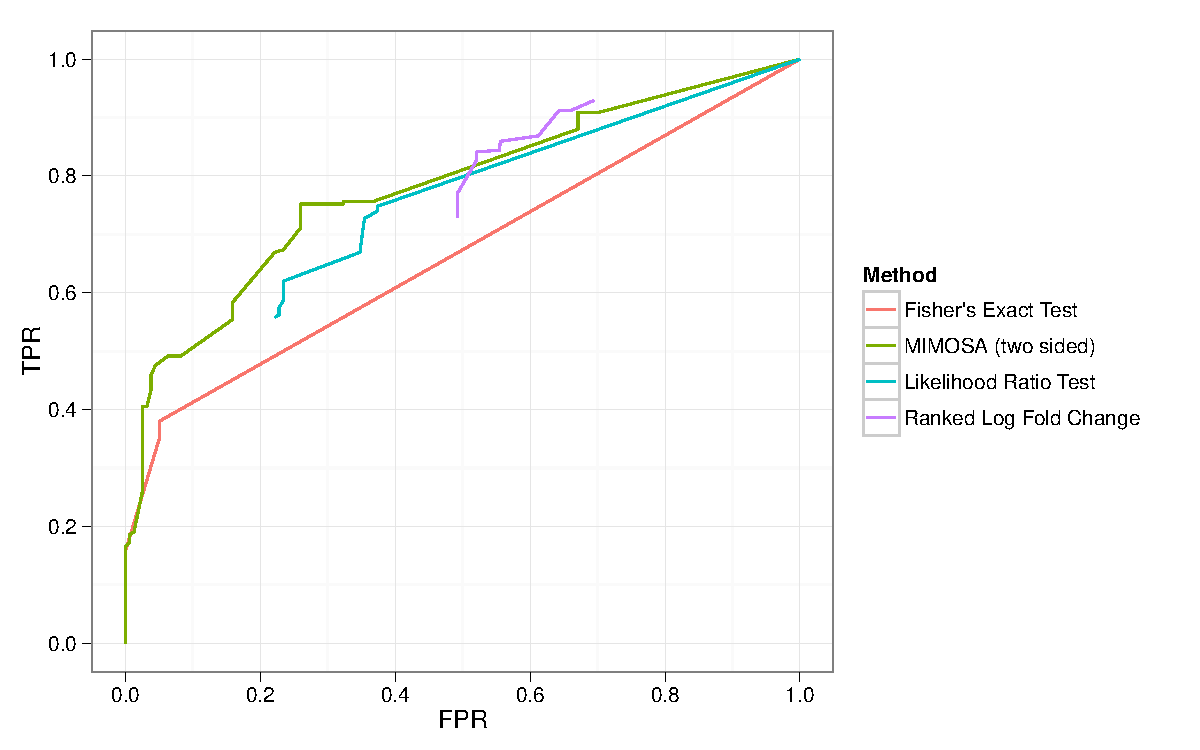
\includegraphics[width=0.4\columnwidth]{Figures/Sim_Twosided_ROC_1000.pdf}};
    \begin{scope} [x={(e.south east)},y={(e.north west)}]
        \node at (0,1) [font=\tiny\sffamily] {E} ;
    \end{scope}
    \end{tikzpicture}
    };
    \node [right=of E] (F) {
    \begin{tikzpicture}
    \node[anchor=south west, inner sep=0] at (0,0) (f) {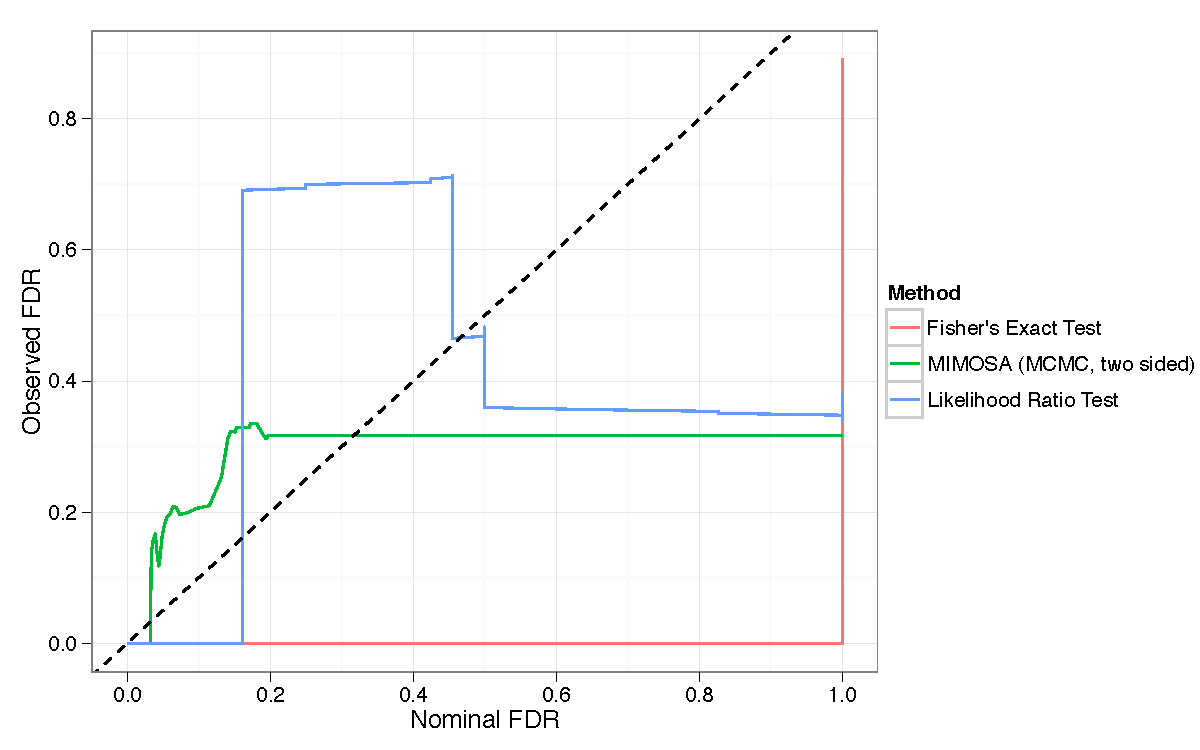
\includegraphics[width=0.4\columnwidth]{Figures/Sim_Twosided_FDR_1000.pdf}};
        \begin{scope} [x={(f.south east)},y={(f.north west)}]
        \node at (0,1) [font=\tiny\sffamily] {F} ;
        \end{scope}
    \end{tikzpicture}
    };
    \node [below=of E] (G) {
    \begin{tikzpicture}
     \node[anchor=south west,inner sep=0] at (0,0) (g) {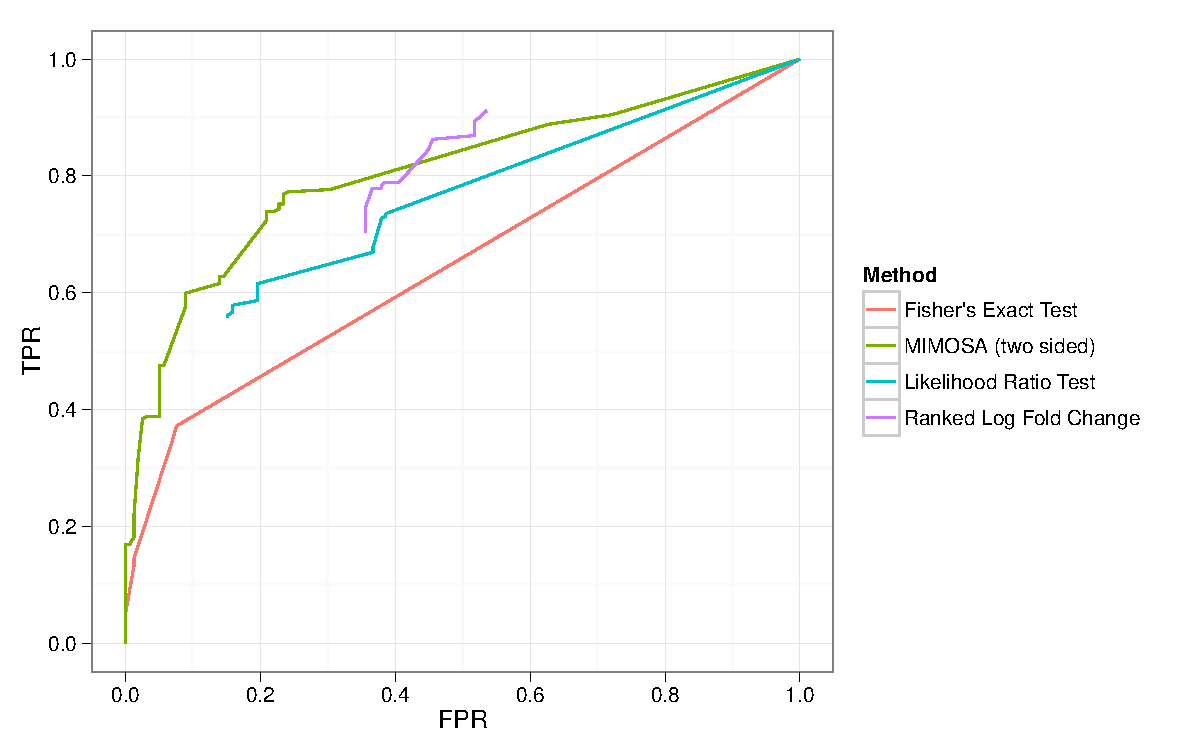
\includegraphics[width=0.4\columnwidth]{Figures/Sim_Truncated_ROC_1000.pdf}};
         \begin{scope} [x={(g.south east)},y={(g.north west)}]
                 \node at (0,1) [font=\tiny\sffamily] {G} ;
	\end{scope}
     \end{tikzpicture}
     };
     \node [below=of F] (H) {
     \begin{tikzpicture}
    \node[anchor=south west, inner sep=0] at (0,0) (h) {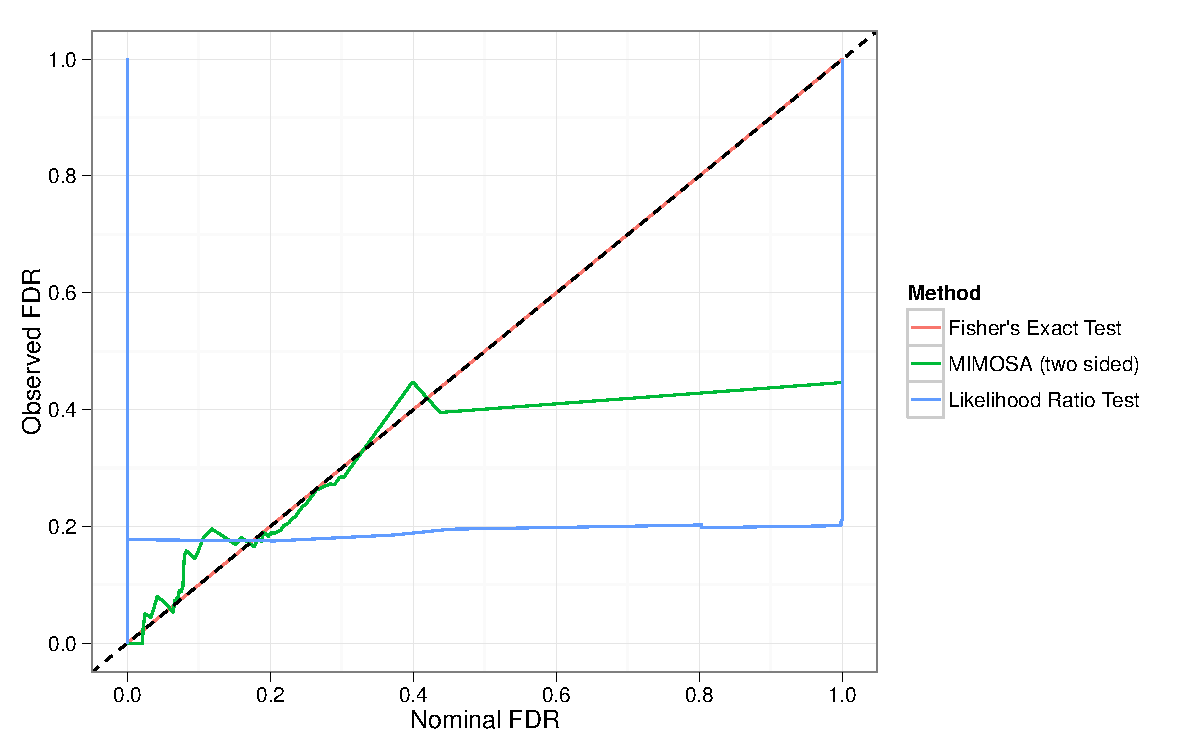
\includegraphics[width=0.4\columnwidth]{Figures/Sim_Truncated_FDR_1000.pdf}};
        \begin{scope} [x={(h.south east)},y={(h.north west)}]
            \node at (0,1) [font=\tiny\sffamily] {H} ;
\end{scope}
    \end{tikzpicture}
    };
 \end{tikzpicture}
   \caption{Unconstrained MIMOSA model fit to two--sided data (A,B,E,F) or to data where model assumptions are violated (C,D,G,H). Two--sided data were simulated from a standard model. A) Average ROC curves and B) average observed vs nominal FDR from 10 simulations with N=5,000, and E-F) N=1,000. Unconstrained MIMOSA fit to two--sided data simulated from a model where the proportions were drawn from a truncated normal distribution over $[0,1]$, rather than a Beta distribution. C) Average ROC curves and D) average observed vs nominal FDR from 10 simulations at N=5,000, and G-H) N=1,000. }
   \label{webfig:simulations_trunc}
\end{figure}
\bibliographystyle{mn2e}
\bibliography{MIMOSA}


\end{document}